\needspace{5\baselineskip}
\chapter{Sincronizzazione tra video e audio}
\label{cha:sync}

Nelle sezioni che seguono viene presentato il problema della sincronizzazione dei flussi video e audio, il cui effetto più evidente è lo sfasamento tra le parole e i movimenti del docente/relatore. I flussi sono acquisiti in modi diversi, per cui la sincronizzazione dell'inizio delle registrazioni non è banale. Viene quindi introdotta una soluzione che sfrutta un marcatore visivo per individuare un punto preciso e condiviso tra le registrazioni, in modo da poterle allineare.

\section{Definizione del problema}
\label{sec:sync_problema}

Come accennato, il problema sorge perché i tre flussi provengono da sorgenti e strumenti di acquisizione diversi. Si tratta in particolare di:

\begin{itemize}
	\item il video dell'ingresso HDMI, registrato con la classe \texttt{MediaRecorder} di Android o eventualmente con SDK dedicati. Nel primo caso si ha un metodo \texttt{start()} che si può prendere come istante approssimativo di inizio della registrazione, ma non è possibile ottenere il \emph{timestamp} preciso di inizio effettivo della registrazione (cioè quello del primo fotogramma);
	\item il video della videocamera IP, registrato con \texttt{ffmpeg} tramite il protocollo RTSP. La latenza di inizio registrazione è difficilmente stimabile, e cioè, in altre parole, dopo l'avvio del comando \texttt{ffmpeg} non è possibile sapere con precisione l'istante a cui corrisponde il primo fotogramma acquisito. La latenza è infatti influenzata da diversi fattori, tra cui la rete, i tempi di codifica, i buffer di trasmissione e di ricezione. Non è quindi facile trovare un intervallo di tempo abbastanza preciso per sincronizzare il video con gli altri flussi;
	\item l'audio di un microfono, collegato via cavo direttamente alla board Android. Questo può essere registrato con la stessa istanza di \texttt{MediaRecorder} del primo punto, ottenendo quindi una sincronizzazione naturale, almeno a livello teorico.
\end{itemize}

A questo punto si ha che le due sorgenti acquisite via cavo (HDMI e audio) sono tra loro sincronizzate, mentre resta il problema di allineare il video RTSP con la traccia audio. Uno sfasamento di anche solo 200-300 millisecondi risulta infatti percepibile e può rendere fastidiosa la fruizione del video.

\section{Proposta di soluzione}
\label{sec:sync_soluzione}

Con le premesse della sezione precedente, una soluzione percorribile è la sincronizzazione tra il video HDMI e il video RTSP, in modo da ottenere transitivamente una sincronizzazione anche con l'audio.

Questo obiettivo è raggiungibile con una ragionevole precisione utilizzando un riferimento visivo che possa essere proiettato su schermo e quindi catturato dalla videocamera. Questo riferimento dovrebbe essere rilevabile in modo automatizzato, in modo da svolgere la funzione di "ciak". Nella pratica potrebbe trattarsi di una schermata verde mostrata per un secondo dall'applicazione, in modo simile alle schermate monocolore utilizzate spesso dai proiettori in caso di assenza di segnale.

La figura \ref{fig:sync1} mostra su una linea del tempo gli intervalli delle registrazioni RTSP e HDMI. Supponiamo in questo caso che la registrazione della videocamera parta per prima, e che la linea verticale indichi l'istante temporale in cui il marcatore visivo viene catturato dalla videocamera. Potrebbe quindi trattarsi del momento in cui la schermata verde compare oppure scompare dalla proiezione.

\begin{figure}[H]
	\centering
	
	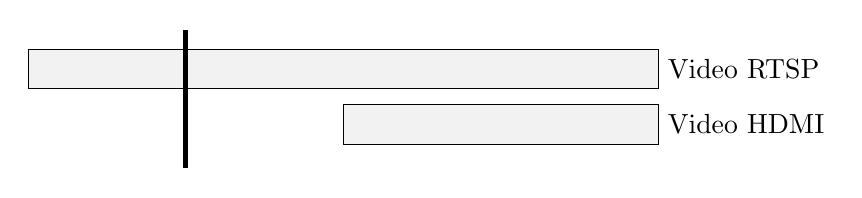
\begin{tikzpicture}
	
	\pgfdeclarelayer{fg}
	\pgfsetlayers{main,fg}
	
	\begin{pgfonlayer}{fg}
	
		\filldraw[fill=black!5,draw=black] (0,0) rectangle ++(8,0.5);
		\node[right] at(8,0.25) {Video RTSP};
		
		\filldraw[fill=black!5,draw=black] (4,-0.7) rectangle ++(4,0.5);
		\node[right] at(8,-0.45) {Video HDMI};
		
		\draw[ultra thick] (2,0.75) -- (2,-1);
	
	\end{pgfonlayer}
	
	\end{tikzpicture}

	\caption{}
	\label{fig:sync1}
\end{figure}

Quello che ci interessa ottenere ora è che le due registrazioni video inizino nello stesso istante della linea del tempo. Dobbiamo quindi tagliare un pezzo del video RTSP in modo che il primo fotogramma RTSP corrisponda al primo fotogramma HDMI. Per farlo ci servono due intervalli di tempo, indicati come A e B nella figura \ref{fig:sync2}.

\begin{figure}[H]
	\centering
	
	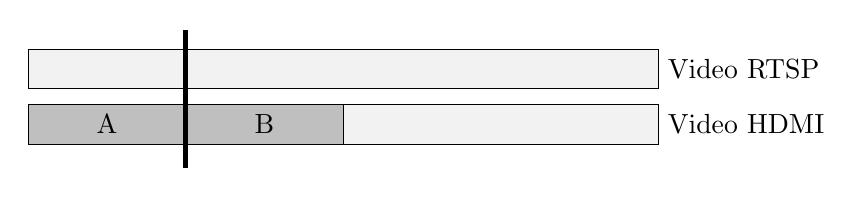
\begin{tikzpicture}
	
	\pgfdeclarelayer{fg}
	\pgfsetlayers{main,fg}
	
	\begin{pgfonlayer}{fg}
	
	\filldraw[fill=black!5,draw=black] (0,0) rectangle ++(8,0.5);
	\node[right] at(8,0.25) {Video RTSP};
	
	\filldraw[fill=black!5,draw=black] (4,-0.7) rectangle ++(4,0.5);
	\node[right] at(8,-0.45) {Video HDMI};
	
	\filldraw[fill=black!25,draw=black] (2,-0.7) rectangle ++(2,0.5) node[midway] {B};
	\filldraw[fill=black!25,draw=black] (0,-0.7) rectangle ++(2,0.5) node[midway] {A};
	
	\draw[ultra thick] (2,0.75) -- (2,-1);
	
	\end{pgfonlayer}
	
	\end{tikzpicture}
	
	\caption{}
	\label{fig:sync2}
\end{figure}

Ottenere l'intervallo B è abbastanza facile, trattandosi di una sottrazione tra \emph{timestamp}. Siamo infatti a conoscenza sia del \emph{timestamp} di avvio della registrazione HDMI sia di quello del riferimento visivo (la linea verticale). L'intervallo B è quindi ottenibile con relativa precisione calcolando la sottrazione tra questi due valori.

L'intervallo A è invece equivalente al tempo trascorso tra l'inizio della registrazione RTSP e l'istante in cui il riferimento visivo compare su schermo. Questo deve essere ricavato analizzando il video tramite strumenti di \emph{computer vision}, come mostrato nella sezione \ref{sec:sync_impl}.

Ottenuti gli intervalli A e B, la loro somma determina lo sfasamento tra video RTSP e HDMI. La rimozione di $(A+B)$ secondi dall'inizio del video RTSP permette quindi di sincronizzare i due flussi video e di conseguenza anche l'audio.

\section{Implementazione e sperimentazione}
\label{sec:sync_impl}

Il primo passaggio per implementare la soluzione è predisporre la visualizzazione del "ciak". Come accennato può trattarsi di una schermata monocolore a schermo intero, ottenibile su Android tramite una \texttt{View} con uno sfondo colorato:

\begin{minted}[highlightlines={8-12}]{xml}
<?xml version="1.0" encoding="utf-8" ?>
<FrameLayout xmlns:android="http://schemas.android.com/apk/res/android"
             xmlns:tools="http://schemas.android.com/tools"
             android:layout_width="match_parent"
             android:layout_height="match_parent"
             tools:context=".MainActivity">

    <View android:id="@+id/rect"
          android:visibility="GONE"
          android:layout_width="match_parent"
          android:layout_height="match_parent"
          android:background="#00ff00" />

</FrameLayout>
\end{minted}

La \texttt{View} è inizialmente nascosta (\texttt{GONE}) e può essere resa visibile via codice così:

\begin{minted}{java}
findViewById(R.id.rect).setVisibility(View.VISIBLE);
\end{minted}

A questo punto è necessario fare uso di timer e ritardi appositamente studiati per ottenere la situazione dello schema della figura \ref{fig:sync1}, cioè fare in modo che la videocamera riprenda il momento in cui la schermata verde viene abilitata.

Passando alla fase di post-elaborazione del materiale acquisito, l'obiettivo principale è riuscire a ricavare dalla registrazione RTSP il tempo in cui compare il marcatore visivo, e cioè l'intervallo A della figura \ref{fig:sync2}. Per fare ciò è possibile usare \texttt{OpenCV}, una nota libreria di visione artificiale.

Più in dettaglio, la tecnica sperimentata consiste nel calcolare la media delle tre componenti di colore RGB per ciascun fotogramma, e di provare poi a rilevare le variazioni significative di verde. Concettualmente, il parametro da considerare per individuare le variazioni è la "distanza" tra il colore verde e le altre componenti di colore, e cioè, in formula, $G - \frac{R+B}{2}$. Il blocco di codice che segue calcola questa distanza per ogni fotogramma del video. 

\inputminted[xleftmargin=\parindent,linenos]{python}{res/opencv.py}

Per comprendere meglio cosa sta succedendo, conviene usare una rappresentazione grafica dei dati raccolti. La figura \ref{fig:sync_opencv1} mostra la variazione nel tempo delle tre coordinate RGB di un video in cui al secondo 6 gran parte dello schermo ripreso diventa verde (figura \ref{fig:sync_video}). Dal grafico è certamente evidente che al secondo 6 c'è un cambiamento significativo e che il valore del verde aumenta leggermente, ma se si osserva meglio non risulta in realtà così facile individuare con precisione e in modo automatizzato l'istante di inizio e fine della schermata verde.

\begin{figure}[htbp]
	\centering
	
	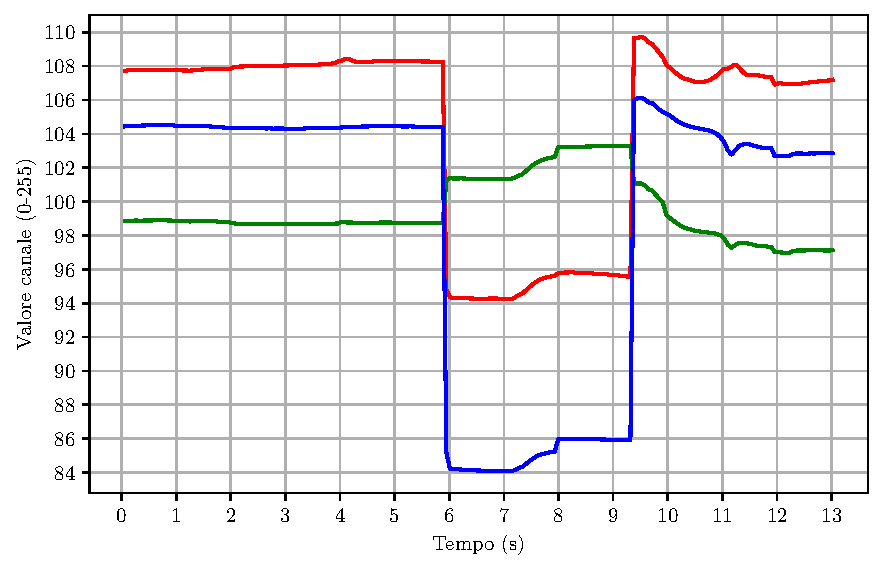
\includegraphics{res/opencv_channels_tight.pdf}
	
	\caption{Variazione delle componenti colore RGB in relazione al tempo.}
	\label{fig:sync_opencv1}
\end{figure}

\begin{figure}[htbp]
	\centering
	
	\begin{subfigure}[t]{0.5\textwidth}
		\centering
		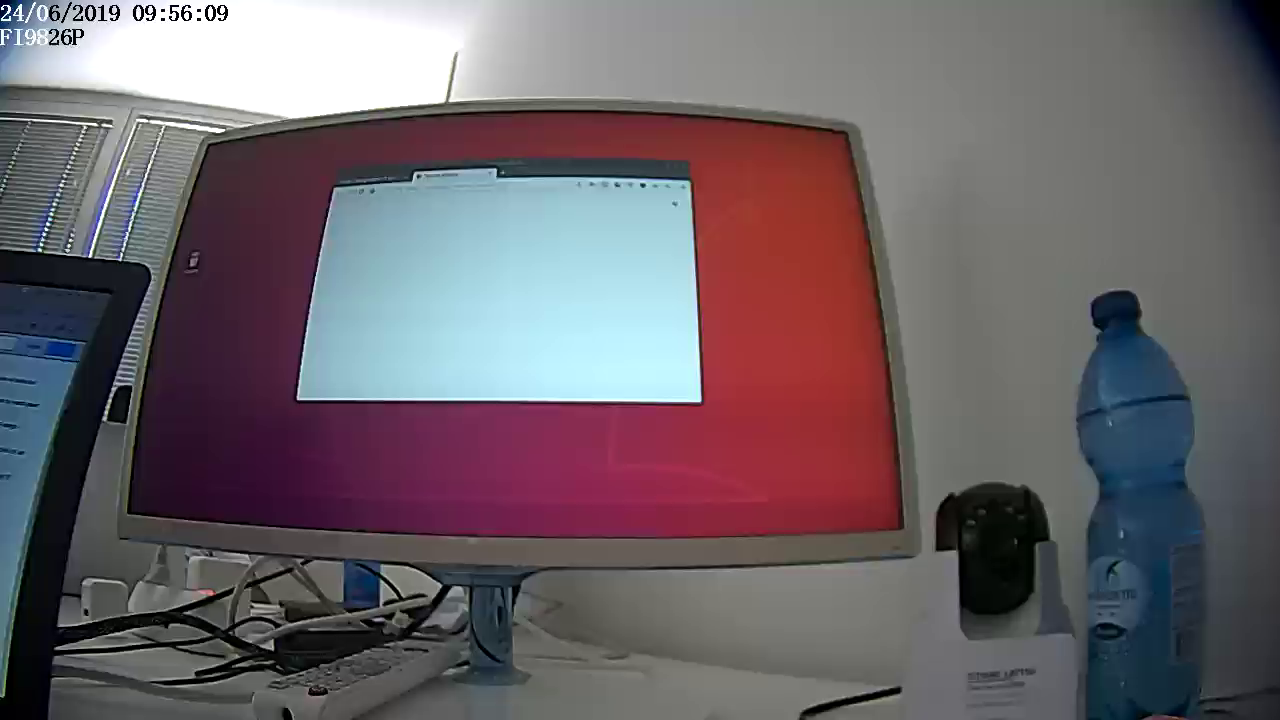
\includegraphics[width=\textwidth]{res/opencv1.png}
		\caption{$t=0s$}
	\end{subfigure}%
	~ 
	\begin{subfigure}[t]{0.5\textwidth}
		\centering
		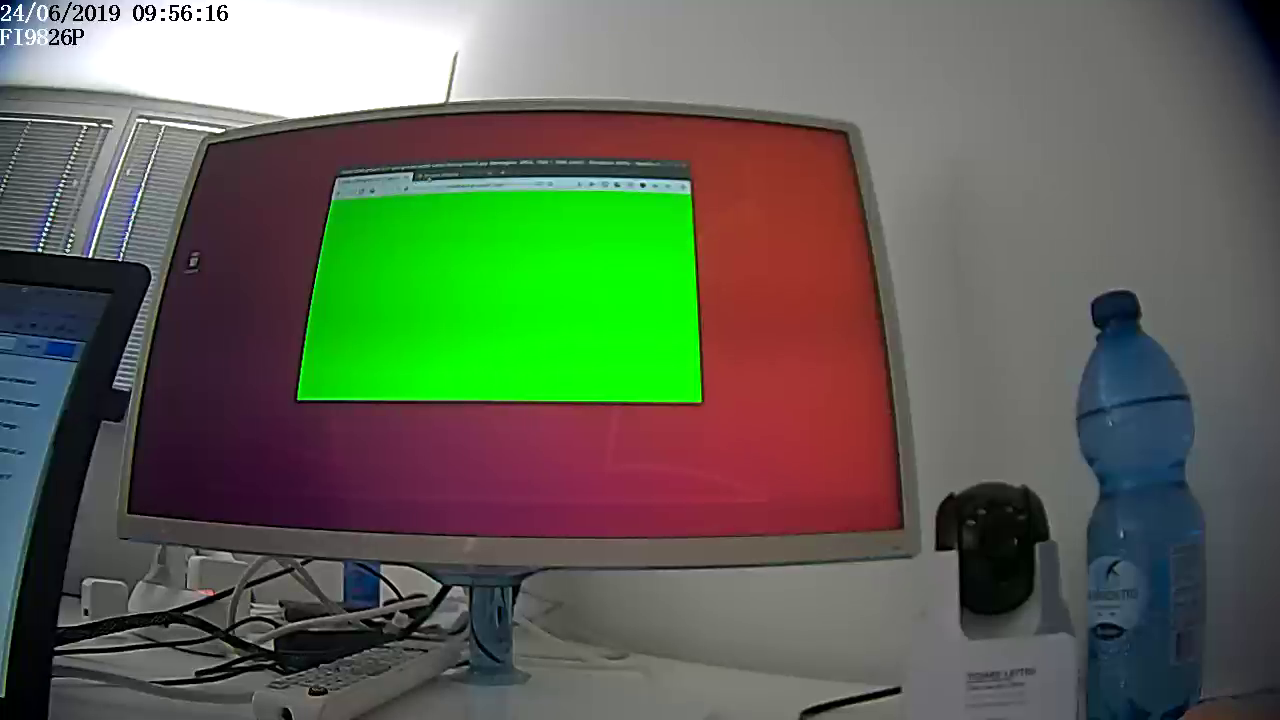
\includegraphics[width=\textwidth]{res/opencv2.png}
		\caption{$t=6s$}
	\end{subfigure}

	\caption{Due fotogrammi del video analizzato, rispettivamente il primo fotogramma e un fotogramma di poco successivo al secondo 6.}
	\label{fig:sync_video}
\end{figure}

La figura \ref{fig:sync_opencv2} mostra invece la distanza tra la componente verde e la media delle altre componenti, come calcolato alla riga 15 dello script Python. Qua il salto è molto più facile da individuare, anche in modo automatizzato, perché si tratta di un delta di quasi 20 che avviene in modo repentino dopo un intervallo di stabilità.

\begin{figure}[htbp]
	\centering
	
	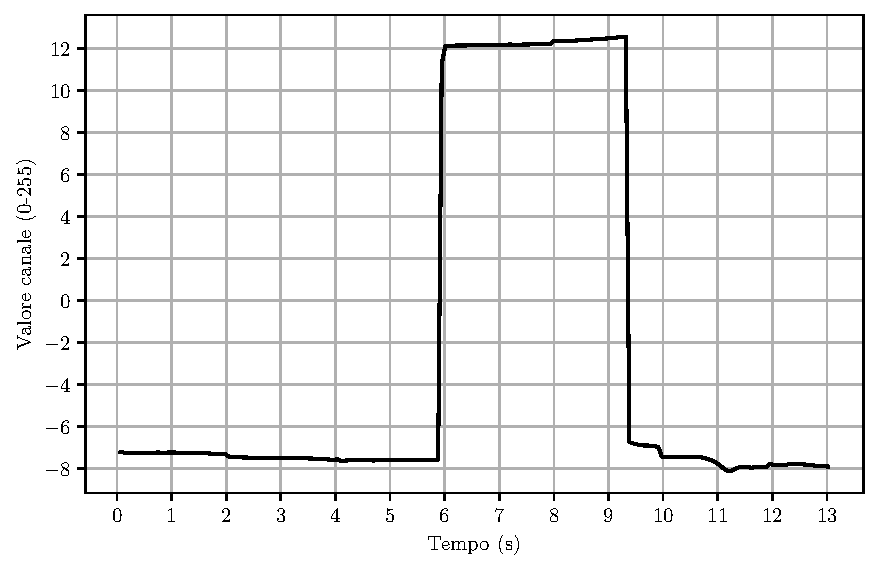
\includegraphics{res/opencv_diff.pdf}
	
	\caption{Variazione della variabile \texttt{diff}, cioè la distanza tra componente verde e la media delle altre componenti, in relazione al tempo.}
	\label{fig:sync_opencv2}
\end{figure}

Per la precisione, la variazione in questo caso avviene leggermente prima del secondo 6, come si evince con evidenza dall'output dello script:

\begin{minted}[highlightlines=5]{text}
[...]
5.747986463620982 => -7.589908854166694
5.81405527354766 => -7.586672634548577
5.880124083474336 => -7.579766167534601
5.946192893401014 => 11.272211914062495
6.012261703327693 => 12.108198242187711
6.078330513254371 => 12.092488064236306
6.144399323181049 => 12.112571614583288
6.210468133107726 => 12.133828125000036
[...]
\end{minted}

È quindi $5,94$ secondi il valore corrispondente all'intervallo A dello schema \ref{fig:sync2}, che può essere sommato a B per ottenere l'intervallo di tempo da tagliare all'inizio del video RTSP.

Supponendo che $A+B$ dia come risultato $8$, possiamo ora ritagliare il video RTSP e ottenere un ragionevole sincronismo tra i due flussi video. Il blocco che segue è una versione minima di un comando che usa \texttt{ffmpeg} per rimuovere i primi 8 secondi del file \texttt{rtsp.mp4}.

\begin{minted}[escapeinside=||]{text}
> ffmpeg |\colorbox{LightCyan}{-ss 8}| -i rtsp.mp4 -r 25 rtsp-synced.mp4 -y
\end{minted}

I risultati ottenuti con questa soluzione sono soddisfacenti, con un disallineamento di circa 70-80 millisecondi a favore del video RTSP. Questo sfasamento pare però essere consistente, ed è probabilmente dovuto al fatto che il \emph{timestamp} memorizzato alla chiamata del metodo \texttt{start()} per l'avvio della registrazione HDMI non è preciso. Questo dipende dal fatto che il metodo \texttt{start()} ritorna istantaneamente, ma la registrazione effettiva inizia in realtà qualche decina di millisecondi dopo. Considerato che questo ritardo è consistente e l'hardware è fisso, una possibilità potrebbe essere di compensarlo manualmente nel calcolo dell'intervallo $A+B$.

